\documentclass{fizykalab}

% Variables
\def\pomvspace{\vspace{0.3em}}

% Ustawienia strony
\usepackage{lipsum}
\usepackage[margin=3cm]{geometry}
\usepackage{graphicx}
\usepackage{enumitem}
\usepackage{siunitx}
\usepackage{amsmath}
\usepackage{cancel}
\usepackage{makecell}
\usepackage{mathtools}
\setlist{leftmargin=15pt,labelindent=15pt}
\setlist[enumerate]{noitemsep,wide=0pt, leftmargin=*}

% Ustawienia stopki
\usepackage{lastpage}
\usepackage{fancyhdr}
\pagestyle{fancy}
\fancyhf{} % sets both header and footer to nothing
\renewcommand{\headrulewidth}{0pt}
\cfoot{\thepage\ z \pageref{LastPage}}

% Ustawienia do tabelki
\wydzial{IEiT}
\autorjeden{Robert Mesek}
\autordwa{}
\rok{II}
\grupa{8 - L}
\zespol{6}
\temat{Kondensatory}
\nrcwiczenia{33}
\datawykonania{24.10.2023}
\dataoddaniajeden{}
\zwrotdopoprawy{}
\dataoddaniadwa{}
\datazaliczenia{}

\begin{document}

\maketitle
{\setlength{\parindent}{0pt}
\section*{Ćwiczenie "33": Kondensatory}
\subsection*{Cel ćwiczenia}
\par
Celem ćwiczenia jest pomiar pojemności kondensatorów powietrznych, z warstwą dielektryka oraz kabla koncentrycznego w celu wyznaczenia stałej elektrycznej $\varepsilon_0$ oraz przenikalności względnych $\varepsilon_r$ różnych materiałów.

\subsection*{Opis ćwiczenia}
\par
Wzór na pojemność kondensatora płaskiego to
\begin{gather*}
	C = \frac{\varepsilon_0 \varepsilon_r S}{d} \text{.}
	\tag{1}
\end{gather*}

Wzór przybliżony na pojemność kondensatora płaskiego z 3 krążkami z pleksi ($\varepsilon_r = 2.6$) to
\begin{gather*}
	C = \frac{\varepsilon_0 (S - 3S_p)}{d} + \frac{\varepsilon_0 \varepsilon_r 3S_p}{d} \\
	\Downarrow \\
	\varepsilon_0 = \frac{Cd}{S + 3(\varepsilon_r - 1)S_p} \text{.}
	\tag{2}
\end{gather*}

Wzór uwzględniający pole rozproszone
\begin{gather*}
	\varepsilon_0 = \frac{4}{\pi}\frac{(Cd)_{extr}}{D^2 + 3(\varepsilon_r - 1) D_p^2}
	\tag{3}
\end{gather*}
\begin{flalign*}
	\text{gdzie: } \quad \quad (Cd)_{extr} \ &- \  \text{ekstrapolowana wartość iloczynu $Cd$} &  & \\
	D \ &- \                                        \text{średnica okładek kondensatora}        &  & \\
	D_p \ &- \                                      \text{średnica przekładki}                  &  & \\
\end{flalign*}

Wzór na $\varepsilon_r$ wykorzystywany do obliczenia pojemności kondensatora cylindrycznego to:
\begin{gather*}
	\varepsilon_r = \frac{C \ln{\frac{R}{r}} }{2\pi \varepsilon_0 l} \text{.}
	\tag{4}
\end{gather*}

\newpage

\section*{Układ pomiarowy}
\par
Układ pomiarowy (Rys. 1) składa się z badanego kondensatora i cyfrowego miernika pojemności elektrycznej.
 
Kondensator składa się z dwóch kołowych płyt aluminiowych o płaskiej powierzchni oraz z przekładek z płyty pleksiglasowej. 

Do pomiarów geometrycznych używamy przymiaru milimetrowego i śruby mikrometrycznej.
 
Do pomiaru pojemności kondensatora służy miernik LCR.
\begin{figure}[!ht]
	\centering
	\vspace{0pt}
	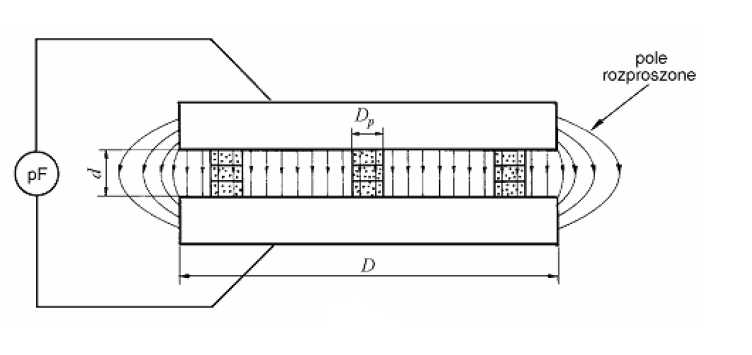
\includegraphics[width=0.9\linewidth]{images/uklad1.png}
	\caption*{Rys. 1 Układ pomiarowy}
\end{figure}



\section*{Przebieg doświadczenia}
\par
Doświadczenie rozpoczniemy od pomiaru długości średnicy okładek kondensatora $D$ za pomocą linijki oraz grubości krążków pleksiglasowych $D_p$ za pomocą śruby mikrometrycznej. 

Następnie przeprowadzimy badanie pojemności, dokładając po jednym krążku w każdym z trzech miejsc, mierząc grubości powstających kolumn. 

Po tym mierzymy pojemności kondensatora z różnymi materiałami użytymi jako rdzeń. 

Ostatecznie zmierzymy pojemność kabla koncentrycznego, który jest kondensatorem cylindrycznym.

\newpage

\section*{Wyniki pomiarów}
\par
\begin{table}[!ht]
	\centering
	\begin{tabular}{|c|c|}
		\hline
		\textbf{Średnica kondensatora [mm]} & \textbf{Średnica przekładki [mm]} \\ \hline
		240 & 20 \\ \hline
	\end{tabular}
	\caption*{Tabela 1a Wymiary kondensatora}
\end{table}

\begin{table}[!ht]
	\centering
	\begin{tabular}{|c|c|c|c|c|c|c|}
		\hline
		\makecell{\textbf{Liczba} \\ \textbf{przekładek}} & \textbf{d1 [mm]} & \textbf{d2 [mm]} & \textbf{d3 [mm]} & \textbf{d [mm]} & \textbf{C [pF]} & \textbf{Cd [mm*pF]} \\ \hline
		1 & 3.83 & 3.83 & 3.84 & 3.83 & 119.30 & 457.32 \\ \hline
		2 & 7.75 & 7.77 & 7.71 & 7.74 & 63.80 & 494.02 \\ \hline
		3 & 11.59 & 11.53 & 11.56 & 11.56 & 44.60 & 515.58 \\ \hline
		4 & 14.55 & 14.44 & 14.43 & 14.47 & 36.90 & 534.07 \\ \hline
		5 & 17.40 & 17.34 & 17.49 & 17.41 & 31.80 & 553.64 \\ \hline
		1 & 3.84 & 3.84 & 3.87 & 3.85 & 119.00 & 458.15 \\ \hline
	\end{tabular}
	\caption*{Tabela 1b Pomiary pojemności dla liczby przekładek}
\end{table}

\begin{table}[!ht]
	\centering
	\begin{tabular}{|c|c|c|c|}
		\hline
		\textbf{Materiał} & \textbf{d [mm]} & \textbf{C [nf]} & \textbf{2R [mm]} \\ \hline
		pleksi & 2.88 & 0.44 & 260 \\ \hline
		pleksi & 9.95 & 0.14 & 267 \\ \hline
		drewno & 12.11 & 0.13 & 240 \\ \hline
		tekstolit & 6.37 & 0.46 & 260 \\ \hline
		PCW & 3.28 & 0.37 & 240 \\ \hline
	\end{tabular}
	\caption*{Tabela 2 Pomiary dla różnych dielektryków}
\end{table}

\begin{table}[!ht]
	\centering
	\begin{tabular}{|c|c|c|c|}
		\hline
		\makecell{\textbf{Średnica}\\\textbf{zewnętrzna [mm]}}  & \makecell{\textbf{Średnica}\\\textbf{wewnętrzna [mm]}} & \textbf{Długość l [mm]} & \textbf{Pojemność kabla C [pF]} \\ \hline
		4.45 & 1.05 & 545 & 35.2 \\ \hline
	\end{tabular}
	\caption*{Tabela 3 Pomiary dla kabla koncentrycznego}
\end{table}

\begin{figure}[!ht]
	\centering
	\vspace{0pt}
	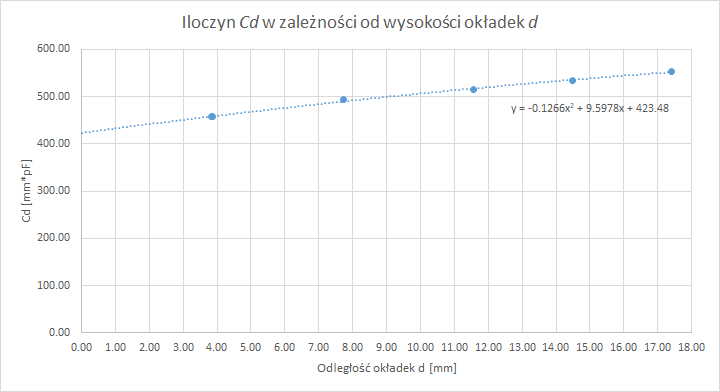
\includegraphics[width=0.6\linewidth]{images/wykres1.png}
	\caption*{Wykres 1 Iloczyn $Cd$ w zależności od wysokości okładek $d$}
\end{figure}

\newpage

\section*{Opracowanie wyników}
\subsection*{Kondensator powietrzny}
\par
Korzystając z programu \textbf{Excel} przeprowadziliśmy krzywą $y = -0.1266x^2 + 9.5978x + 423.48$ przez punkty oraz ekstrapolowana wartość dla $d = 0$ to: 
\[ (Cd)_{extr} = 423.48 \ \text{mm}\cdot\text{pF} \approx 0.42 \ \text{m}\cdot\text{pF}\]
oraz
\[ u((Cd)_{extr})  = 23.96 \ \text{mm}\cdot\text{pF}\ \approx 0.02 \ \text{m}\cdot\text{pF} \]

Wartość stałej elektrycznej wyliczona ze wzoru (3):
\[ \varepsilon_0 = 8.98 \ \frac{\text{pF}}{\text{m}} \]

Prawo przenoszenia niepewności dla wzoru (3)
\[ U(D) = 1 \ \text{mm} \]
\begin{gather*}
	u(\varepsilon_0) = \sqrt{\left(\frac{\partial \varepsilon_0}{\partial (Cd)_{extr}}\cdot u((Cd)_{extr})\right)^2 + \left(\frac{\partial \varepsilon_0}{\partial D}\cdot u(D)\right)^2} = \\
	= \sqrt{\left(\frac{4}{\pi D^2}\cdot u((Cd)_{extr})\right)^2 + \left(\frac{8 (Cd)_{extr}}{\pi D^3}\cdot u(D)\right)^2} = 0.45 \ \frac{\text{pF}}{\text{m}}
	\tag{5}
\end{gather*}

Ostatecznie:
\begin{gather*} 
	\boxed{\varepsilon_0 = 8.98 \pm 0.45 \ \frac{\text{pF}}{\text{m}} }
\end{gather*}

\subsection*{Prędkość światła}
\par Aby obliczyć prędkość światła wykorzystamy wzór na prędkość światła w próżni:
\begin{gather*} 
	c = \frac{1}{\sqrt{\varepsilon_0 \mu_0}}
	\tag{6}
	\end{gather*}
Stała magnetyczna jest równa $ 4\pi \cdot 10^{-7} \ \frac{N}{A^2}$

Po podstawieniu
\[ c \approx 297 \ 684 \ 964 \ \frac{m}{s}\]

Niepewności prędkości światła
\[ u(c) = \sqrt{\left(\frac{dc}{d\varepsilon_0} u(\varepsilon_0)\right)^2} = \left|\frac{u(\varepsilon_0)}{\sqrt{\varepsilon_0^3 \mu_0}}\right| \approx 14 \ 900 \ 000 \ \frac{m}{s}\]

Ostatecznie:
\begin{gather*} 
	\boxed{c = 297 \ 684 \ 964 \pm 14 \ 900 \ 000 \ \ \frac{\text{m}}{\text{s}} }
\end{gather*}

\newpage

\subsection*{Kondensator z dielektrykiem i kabel koncentryczny}
\par
Przekształcając wzór (1) otrzymujemy wzór na przenikalność elektryczną:
\begin{gather*} 
	\varepsilon_r = \frac{Cd}{\varepsilon_0 S}
	\tag{7}
\end{gather*}
\iffalse % COMMENT
\par
Prawo przenoszenia niepewności:
\[ u(d) = 0.01 \ \text{mm} = 0.00001 \ \text{m} \]
\[ u(S) = 1 \ \text{mm} = 0.001 \ \text{m} \]
\[ u(C) = 0.01 \ \text{nF} = 1 \cdot 10^{-11} \ \text{F} \]

\begin{gather*} 
	u(\varepsilon_r) = \sqrt{\left( \frac{\partial \varepsilon_r}{\partial d} \cdot u(d) \right)^2 + \left(\frac{\partial \varepsilon_r}{\partial S} \cdot u(S)\right)^2 + \left(\frac{\partial \varepsilon_r}{\partial C} \cdot u(C)\right)^2} = 
\end{gather*}
\fi
Otrzymane wzory (4) dla kondensatora cylindrycznego i (7) dla kondensatora płaskiego wykorzystaliśmy do obliczenia przenikalności elektrycznej:
\begin{table}[H]
	\centering
	\begin{tabular}{|c|c|c|c|c|}
		\hline
		\textbf{Materiał} & $\boldsymbol{\varepsilon_r}$ \\ \hline
		kabel koncentryczny & 1.68 \\ \hline
		pleksi & 3.16 \\ \hline
		pleksi & 3.48 \\ \hline
		drewno & 3.93 \\ \hline
		tekstolit & 7.32 \\ \hline
		PCW & 3.03 \\ \hline
	\end{tabular}
	\caption*{Tabela 4}
\end{table}

\section*{Wnioski}
\par
Zgodnie z przewidywaniami uzyskane wyniki są zgodne z tabelaryczną stałą $\varepsilon_0 = 8.854 \ \frac{pF}{m}$.

 Dzięki dokładnemu wyznaczeniu wartości $\varepsilon_0$ mogliśmy obliczyć z dużą dokładnością prędkość światła.
 
 
Obliczone niepewności pomiarowe najprawdopodobniej wynikały z niedoskonałości przyrządów pomiarowych.

Wartości przenikalności elektrycznej dla poszczególnych materiałów zdają się być podobne do wartości tabelarycznych.

\end{document}
